\chapter{The Container Loading Problem}
\label{sec:clp_definition}

The placement and assignment of items to larger, mostly rectangular
containers, is a well known problem in logistics and operations research, as the
potential of cost savings and efficiency gains is substantial by reducing the number
of needed containers or by fulfilling customer needs. The \gls{CLP} covers a broad range of real-world applications,
such as loading cargo, optimizing warehouse storage and packing of pallets or cardboard boxes.
Generally is is differentiated in \textit{input minimization},
where the number of needed containers is minimized, and \textit{output maximization} problems,
where the value of the associated items is maximized. The \gls{BPP} belongs to \textit{input minimization} problems
and the Knapsack Problem to \textit{output maximization}. Apart from the expected outcome of the optimization,
the characterics of the items and containers is crucial for the problem definition. Items can be either
homogeneous or heterogeneous in size and shape. Furthermore, they can be classified as weakly or strongly
homogeneous or heterogeneous, depending on the degree of similarity among them. The container is
defined as a recangular volume with a fixed size and shape, where the items have to be placed in.
Other, non rectangular, shapes are seldomly considered in the literature, as the practical relevance is
limited. Multiple containers of homogeneous or heterogenous sizes are used when the volume and weight
of the cargo require it\footcite[cf.][pp.1--2]{bortfeldt_constraints_2013}.
According to \citeauthor*{bischoff_issues_1995}, the mere placement of items is insufficient
if practical requirements are not fulfilled as it lacks practical applicability \footcite[cf.][pp.1--2]{bischoff_issues_1995}.
\citeauthor*{bortfeldt_constraints_2013} systematically categorized all constraints related
to the \gls{CLP} into five groups, which are presented in the following. They also distinguish between hard and soft constraints,
where hard constraints must be strictly satisfied, while soft constraints may be violated
to some extent \footcite[cf.][p.2]{bortfeldt_constraints_2013}.

\subsubsection{Container related constraints}
These constraints summarize all physical barriers of the container. The \textbf{load capacity} limits the aggregated
mass of all items in the container. The distribution of the weight (\textbf{load balance})
plays an important role for safety reasons, as the cargo must not move during the transport and the container
must not tip over and is defined by the maximum weight difference between the left and right half of the container.
When trucks are transporting the containers, uneven \textbf{axle weight} distribution can cause severe
consequences and need to be avoided by loading the cargo axle-friendly \footcite[cf.][pp. 849--850]{krebs_advanced_2021}.

\subsubsection{Item related constraints}
Item related constraints define the properties of the item, which are relevant
for the packing. When the container capacity is limited (\textit{output maximization}),
the \textbf{loading priority} constraint defines the priority among possible
item candidates. The \textbf{orientation} constraint restricts how an item can be rotated.
Several rotation types exist, each defined by the axis around which the item can rotate.
The most common is the \textbf{z-rotation}, where rotation is only allowed around the vertical axis.
When 3D packing is considered, stacking of items is allowed in comparison to 2D packing, when all
items are placed on the container floor. Two stacking constraint approaches exist.
The \textbf{fragility} constraint differentiates between \textit{fragile} and \textit{non-fragile} items,
allowing only non-fragile items to be stacked on non-fragile items. Figure \ref{fig:stacking_comparison} showcases
this definition. The other approach defines an individual \textit{load-bearing strength} (\textbf{LB Strength}) for each
item stating how much pressure the box can tolerate, and which items can be stacked \footcite[cf.][pp. 847--848]{krebs_advanced_2021}.

\begin{figure}[htbp]
    \centering
    % First TikZ picture
    \begin{subfigure}[b]{0.45\textwidth}
        \centering
        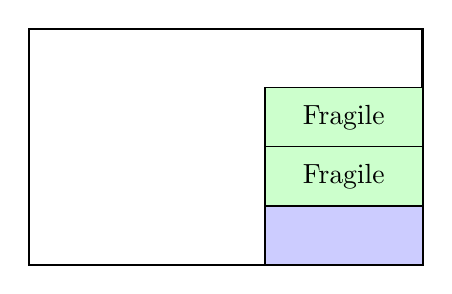
\begin{tikzpicture}
            % Draw the container
            \draw[thick] (0,0) rectangle (5,3);

            % Draw the three items inside
            \draw[fill=blue!20] (3,0) rectangle (5,0.75);
            \node at (4, 0.5) {};

            \draw[fill=green!20] (3,0.75) rectangle (5,1.5);
            \node at (4, 1.125) {Fragile};

            \draw[fill=green!20] (3,1.5) rectangle (5, 2.25);
            \node at (4, 1.875) {Fragile};

        \end{tikzpicture}
        \caption{Feasible stacking of items}
    \end{subfigure}
    \hfill
    % Second TikZ picture
    \begin{subfigure}[b]{0.45\textwidth}
        \centering
        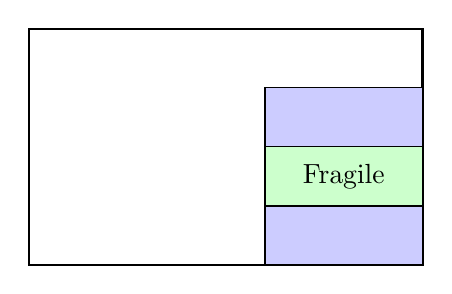
\begin{tikzpicture}
            \draw[thick] (0,0) rectangle (5,3);

            % Draw the three items inside
            \draw[fill=blue!20] (3,0) rectangle (5,0.75);
            \node at (4, 0.5) {};

            \draw[fill=green!20] (3,0.75) rectangle (5,1.5);
            \node at (4, 1.125) {Fragile};

            \draw[fill=blue!20] (3,1.5) rectangle (5, 2.25);
            \node at (4, 1.875) {};
        \end{tikzpicture}
        \caption{Infeasible stacking of items}
    \end{subfigure}
    \caption[Visualization fragile stacking]{Comparison fragile stacking \footnotemark}
    \footnotetext{Own figure}
    \label{fig:stacking_comparison}
\end{figure}


\subsubsection{Cargo-Related Constraints}
In contrast to item-related constraints, cargo-related constraints apply to
the entire cargo or to specific subsets of it. The \textbf{complete-shipment} constraint
requires that all items within a shipment must either be loaded into the same
container or be left behind entirely. This constraint is important
when container capacity is limited (\textit{output maximization}) and items
cannot be split. The \textbf{allocation constraint} serves a similar purpose,
including the \textbf{connectivity constraint}, which mandates that
certain items must be loaded into the same container, and the
\textbf{separation constraint}, which requires specific items to
be distributed across different containers. For example, kitchen
shipments, comprising multiple packages, should be delivered together
to enable efficient installation. Conversely, items such as perfume and fresh
vegetables should be shipped separately due to incompatibility.

\subsubsection{Positioning constraints}

Positioning constraints determine, if items must be placed at
absolute locations or relative to other items. Absolute positioning is
typically based on item characteristics such as size, weight, or
content (e.g., bulky or hazardous items placed near the container door for accessibility) or
they may universally apply to all items, as the \textbf{geometry} and
\textbf{orthogonality} constraints. These constraints define that items are not allowed to overlap
and must be placed orhogonally to thxwe container walls respectively.
Relative positioning requires items to be placed either close together as a \textit{group} or
\textit{separated} from one another.
The \textbf{multi-drop constraint} combines absolute and relative positioning requirements for items
destined for different delivery locations. It aims to minimize reloading efforts by grouping items
by destination, arranging these groups according to the delivery sequence, and/or applying a \textbf{\gls{LIFO}} or
sequential loading policy to ensure efficient unloading without the need to move unrelated items.
Variations of the \gls{LIFO} constraint account for manual unloading (\textbf{\gls{MLIFO}}) or unloading based on the
maximum allowable distance from the unloading point (\textbf{reachability constraint}). Figure~\ref{fig:solution-visualization}
visualizes a possible 3D packing with different constraints applied.

\begin{figure}[ht]
    \centering
    \includegraphics[width=6.3cm]{pictures/3l_cvrp_example.png}
    \caption[Visualized 3D packing with packing constraints]{3D Packing with geometry, orthogonality and support area constraints\footnotemark}.
    \footnotetext{CLP Visualizer from \cite{tamke_branch-and-cut_2024}}
    \label{fig:solution-visualization}
\end{figure}

\subsubsection{Load-related constraints}

The \textbf{stability constraint} is defined as one of the most critical constraints
in the \gls{CLP}, as it directly impacts the safety of both the cargo and the personnel involved.
First, a distinction must be made between \textit{horizontal} and \textit{vertical} stability.
Horizontal stability is achieved when items are securely connected to the
container walls or to other items, preventing lateral movement. Vertical
stability, on the other hand, is defined in various ways throughout the
literature. A common approach to assessing vertical stability is through the concept of the \textbf{support
    area}, the portion of an item's base that rests on the surface below. Stability is typically
considered sufficient when the support area covers $70\%$ to $100\%$ of the item’s base \footcite[cf.][p.344]{gendreau_tabu_2006} However,
this may still result in unstable configurations if the center of gravity falls outside the
support area of the underlying layers, potentially causing the cargo to tilt. To improve robustness,
a more reliable definition of vertical stability requires a minimum support area for all items below,
referred to as \textbf{Robust Stability} \footcite[cf.][p.1140]{ceschia_local_2013}. This comparison is illustrated in Figure~\ref{fig:vertical_stability_comparison}.
Additionally, it is crucial to ensure that the load remains stable even after partial unloading.
In addition, \textbf{complexity constraints} refer to specialized
requirements that are beyond standard packing rules. These include, for example, compatibility with automated or robot-assisted packing systems.

\begin{figure}[htbp]
    \centering
    % First TikZ picture
    \begin{subfigure}[b]{0.45\textwidth}
        \centering
        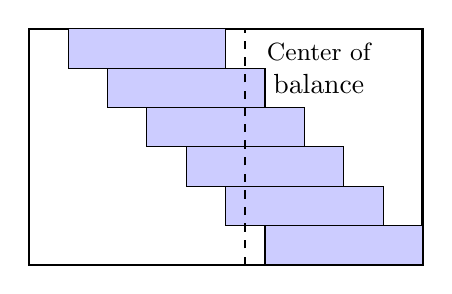
\begin{tikzpicture}
            % Draw the container
            \draw[thick] (0,0) rectangle (5,3);

            % Draw the three items inside
            \draw[fill=blue!20] (3,0) rectangle (5,0.5);
            \draw[fill=blue!20] (2.5,0.5) rectangle (4.5,1);
            \draw[fill=blue!20] (2,1) rectangle (4, 1.5);
            \draw[fill=blue!20] (1.5,1.5) rectangle (3.5, 2);
            \draw[fill=blue!20] (1,2) rectangle (3, 2.5);
            \draw[fill=blue!20] (0.5,2.5) rectangle (2.5, 3);
            %\node at (4, 1.875) {Fragile};
            \draw[thick,dashed] (2.75,0) -- (2.75,3);  % <---
            \node[anchor = west,align=center] at (2.9,2.5) {\small Center of \\  balance};

        \end{tikzpicture}
        \caption[align = center]{Feasible stacking with 75\% support area; infeasible due to unstable center}
    \end{subfigure}
    \hfill
    % Second TikZ picture
    \begin{subfigure}[b]{0.45\textwidth}
        \centering
        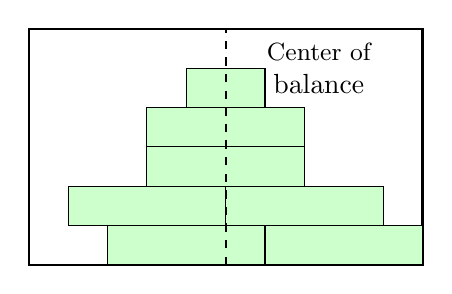
\begin{tikzpicture}
            % Draw the container
            \draw[thick] (0,0) rectangle (5,3);

            % Draw the three items inside
            \draw[fill=green!20] (3,0) rectangle (5,0.5);
            \draw[fill=green!20] (1,0) rectangle (3,0.5);

            \draw[fill=green!20] (2.5,0.5) rectangle (4.5,1);
            \draw[fill=green!20] (0.5,0.5) rectangle (2.5,1);

            \draw[fill=green!20] (1.5,1) rectangle (3.5, 1.5);
            \draw[fill=green!20] (1.5,1.5) rectangle (3.5, 2);
            \draw[fill=green!20] (2,2) rectangle (3, 2.5);

            \draw[thick,dashed] (2.5,0) -- (2.5,3);  % <---
            \node[anchor = west,align=center] at (2.9,2.5) {\small Center of \\  balance};
        \end{tikzpicture}
        \caption[align = center]{Feasible stacking regarding 75\% support area and stable center}
    \end{subfigure}
    \caption[Visualization vertical stability]{Comparison vertical stability (side view) \footnotemark}
    \footnotetext{Own figures based on \cite[p.845]{krebs_advanced_2021}}
    \label{fig:vertical_stability_comparison}
\end{figure}
